\appendix

\section{Theoretical sequences}\label{sec:appendix_sequences}
    We have different sequences that are possible in a theory but will never happens in real cases scenarios. Those cases generally implies that the two springs have exactly the same stiffness. We can see those sequences on Figure \ref{fig:sequence_impossible}. They all require two blocks to displace at the same time and in the same direction. Although they are not possible in real life, they are implemented in the simulation.
    
    \begin{figure}
    \centering
        \begin{tabular}{ccc}
            \subfloat[Sequence K]{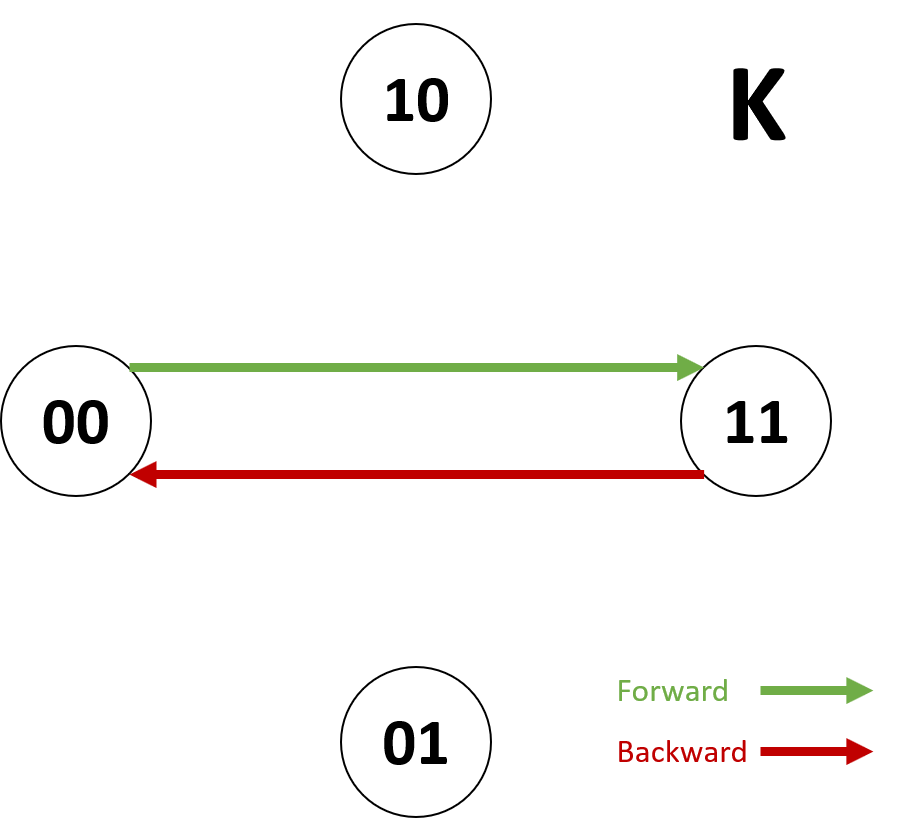
\includegraphics[width = 1.5in]{images/S_K.png}} &
            \subfloat[Sequence L]{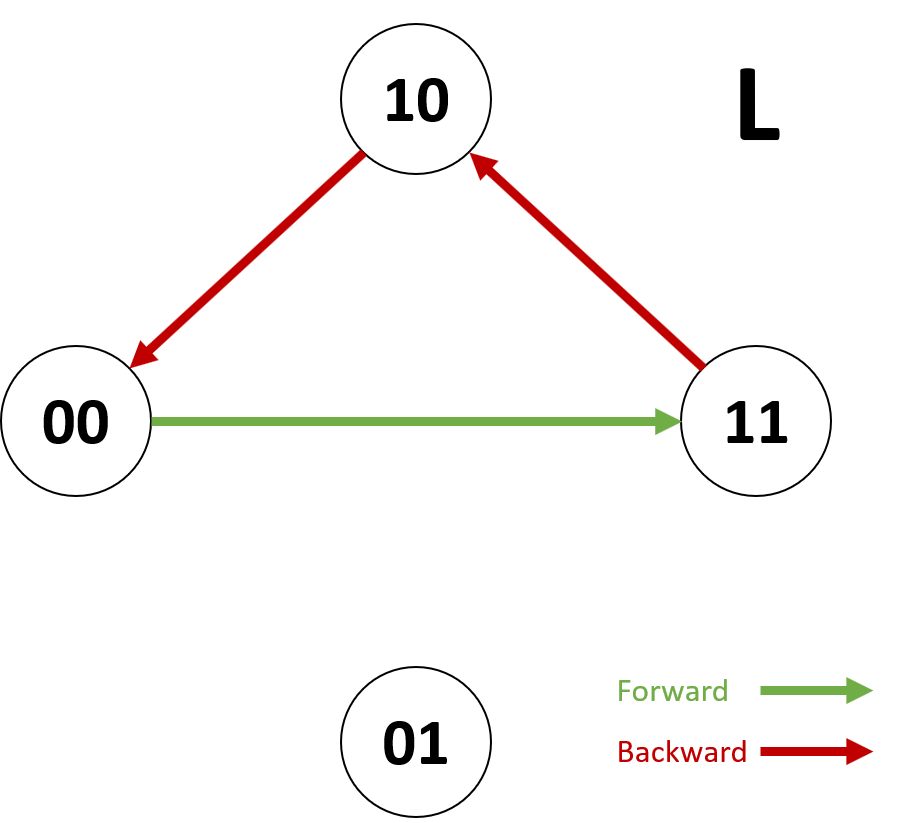
\includegraphics[width = 1.5in]{images/S_L.png}} &
            \subfloat[Sequence M]{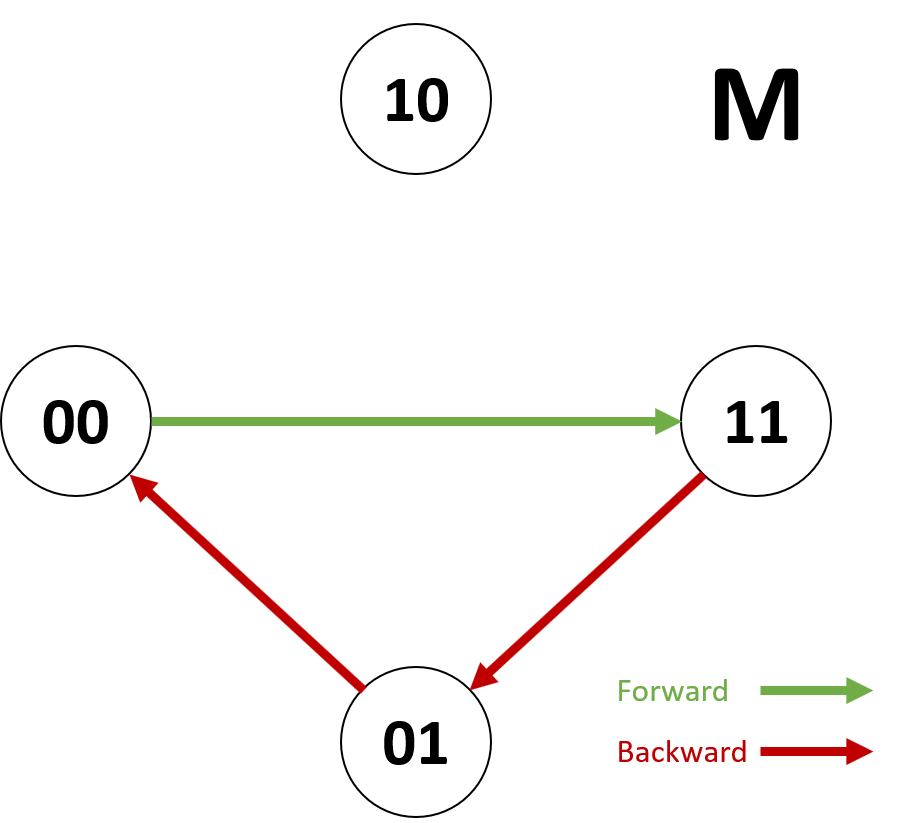
\includegraphics[width = 1.5in]{images/S_M.png}} \\
            \subfloat[Sequence N]{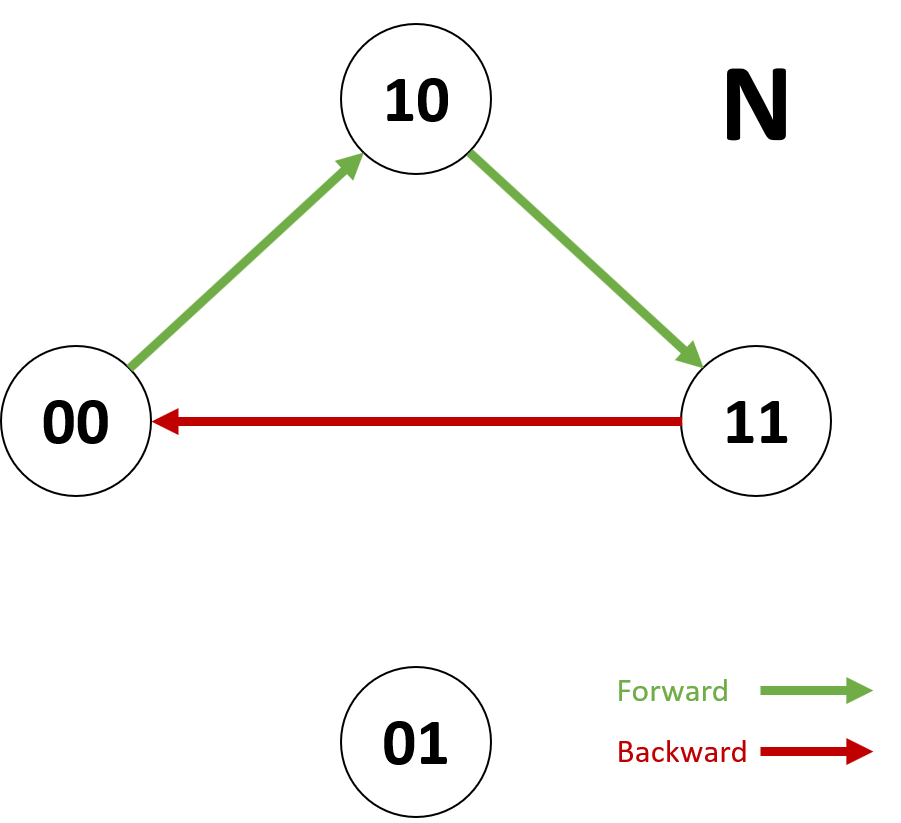
\includegraphics[width = 1.5in]{images/S_N.png}} &
            \subfloat[Sequence O]{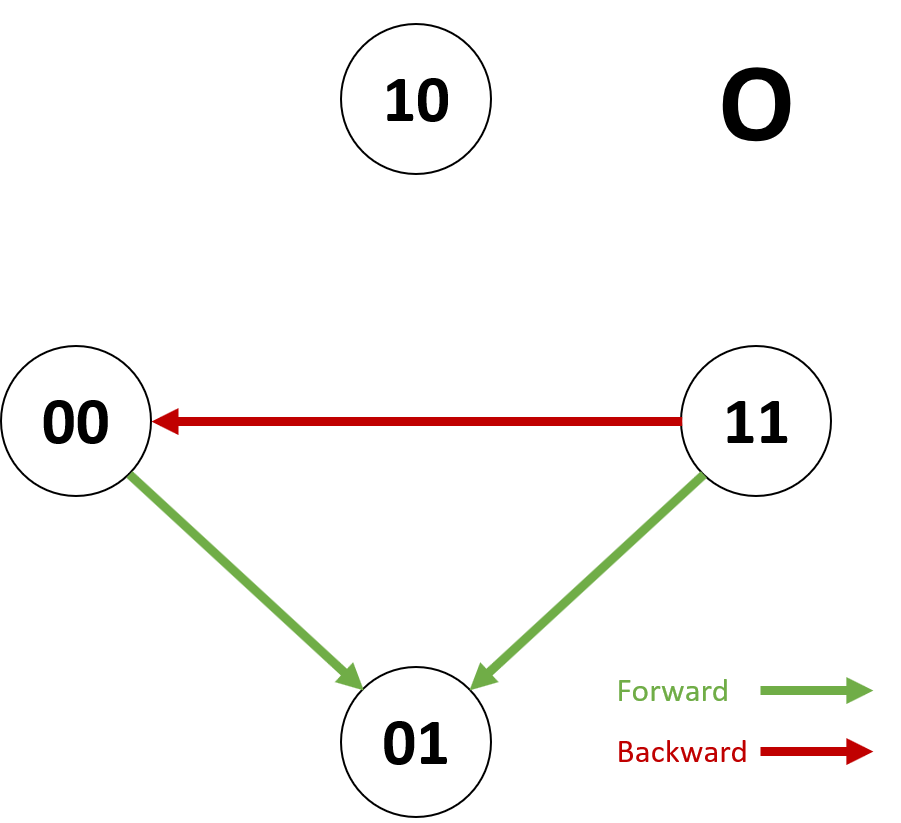
\includegraphics[width = 1.5in]{images/S_O.png}} &
        \end{tabular}
        \caption{Theoretical sequences of the multistable joint that are not possible in real life as it asks to have perfectly balanced springs and same friction in all the joints.}
        \label{fig:sequence_impossible}
    \end{figure}